\documentclass[12pt]{article}

% Packages
\usepackage[margin=1in]{geometry}
\usepackage{amsmath,amssymb,amsthm}
\usepackage{enumitem}
\usepackage{hyperref}
\usepackage{xcolor}
\usepackage{import}
\usepackage{xifthen}
\usepackage{pdfpages}
\usepackage{transparent}
\usepackage{listings}


\lstset{
    breaklines=true,         % Enable line wrapping
    breakatwhitespace=false, % Wrap lines even if there's no whitespace
    basicstyle=\ttfamily,    % Use monospaced font
    frame=single,            % Add a frame around the code
    columns=fullflexible,    % Better handling of variable-width fonts
}

\newcommand{\incfig}[1]{%
    \def\svgwidth{\columnwidth}
    \import{./Figures/}{#1.pdf_tex}
}
\theoremstyle{definition} % This style uses normal (non-italicized) text
\newtheorem{solution}{Solution}
\newtheorem*{proposition}{Proposition}
\newtheorem{problem}{Problem}
\newtheorem{lemma}{Lemma}
\theoremstyle{plain} % Restore the default style for other theorem environments
%

% Theorem-like environments
% Title information
\title{Plan for Winter 2024 Finals}
\author{Jerich Lee}
\date{\today}

\begin{document}

\maketitle
So I have a lot to do this winter, but I honestly feel pretty good about it. ChatGPT will be my good friend and will be doing a lot of the heavy lifting for me, which is 
great. I spent a good amount of time in Boston just thinking and reflecting about this winter, and I feel pretty good about it.
\vspace{.5cm} 
I am going to utilize the tool that I built this summer, Aeren. It's basically just an interface for me to keep track of myself and other things, like tasks, food, and such. It's not really
meant to be like an all-encompassing thing for \emph{every} little detail in my life, but it's a good way for me to just stay on track while trying to balance so many things at once.
\begin{figure}[htbp]
    \centering
    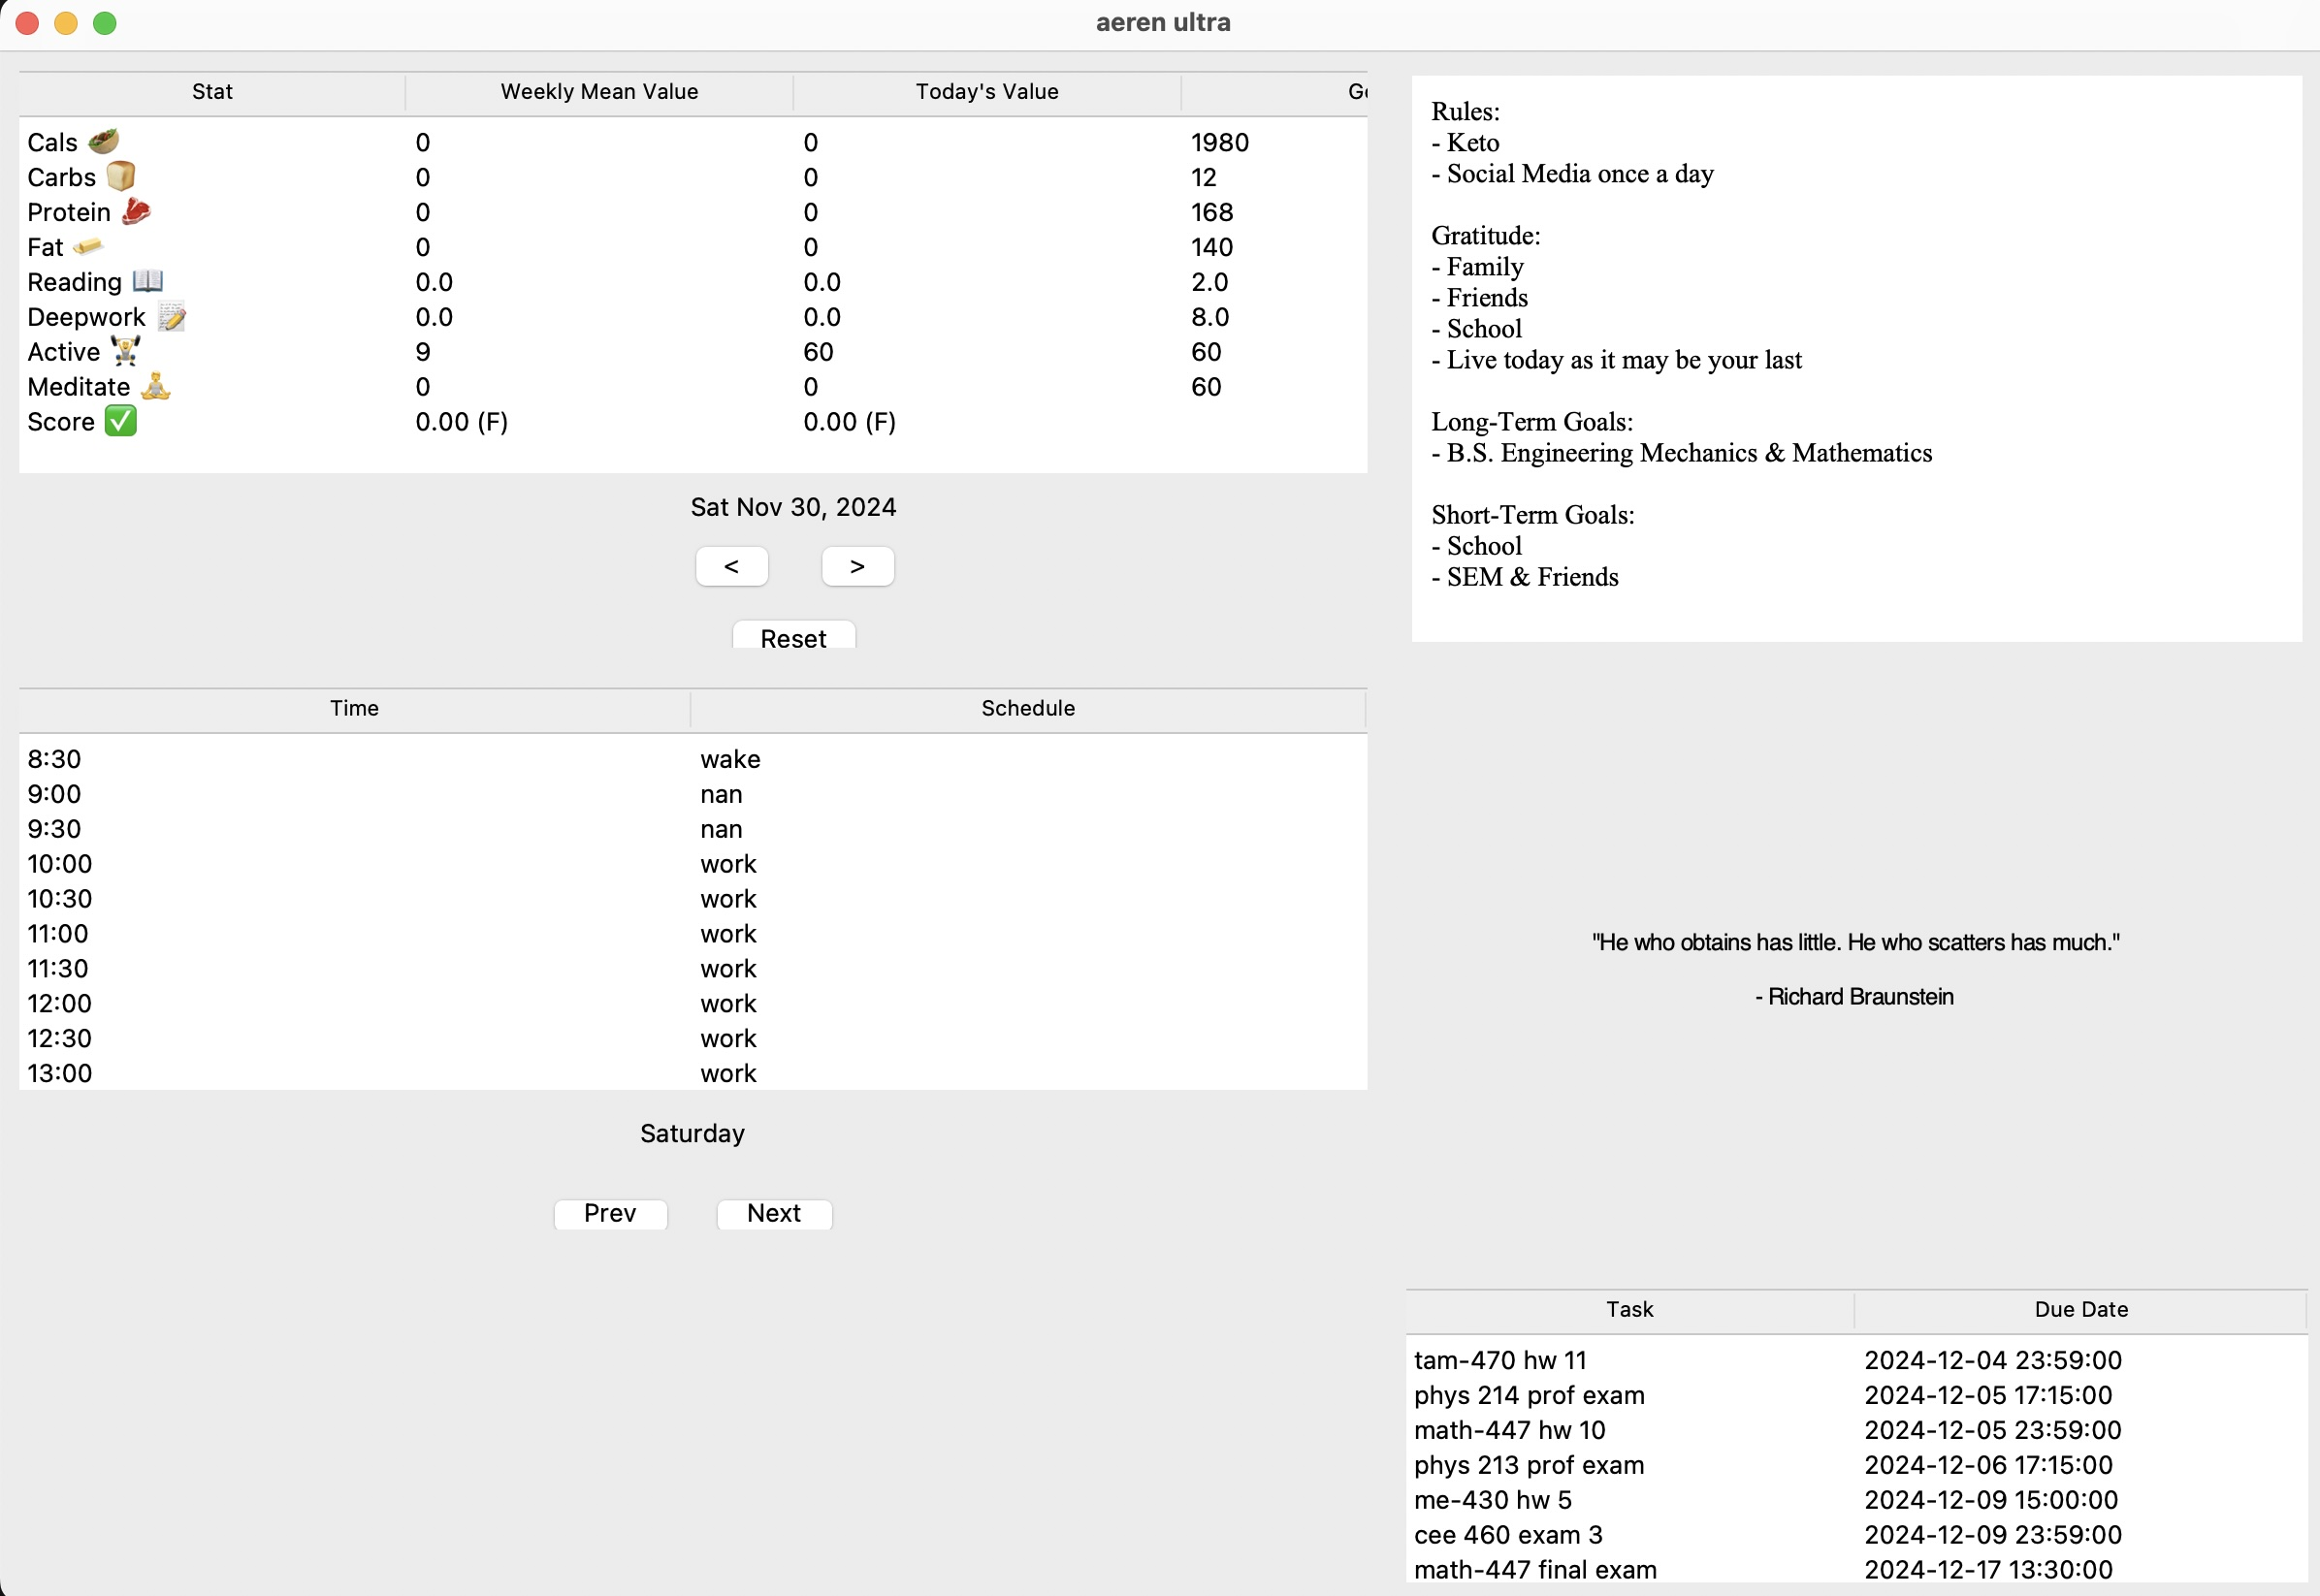
\includegraphics[width=0.8\textwidth]{/Users/jerichlee/Documents/jerichlee.ai/blog/assets/aeren_ultra.jpg}
    \caption{My program!} 
    \label{fig:}
\end{figure}
I'm going to work hard this winter and make myself proud. Let's get this work done.
\vspace{.5cm} 
\subsection{Goals:}
\subsubsection{prof exams}
   \begin{enumerate}
    \item phys 213
    \item phys 214
    \item math 220
    \item chin 203
   \end{enumerate}
   \subsubsection{class finals}
   \begin{enumerate}
    \item math 447
    \item tam 470
    \item me 430
    \item cee 460
   \end{enumerate}
   \subsubsection{jobs}
   \begin{enumerate}
    \item apply every weekend...or dad will not be very happy with you at break... 
   \end{enumerate}
   \vspace{.5cm}  
   \subsection{Manifesting}
   \subsubsection{Spring 2025:}
   \begin{enumerate}
    \item math 448
    \item math 432
    \item math 417
    \item me 470
    \item job secured???
    \item \begin{enumerate}
        \item pay off school
        \item become independent
        \item work for a couple and apply to grad school in math :‑O
        \item \begin{enumerate}
            \item get my graduate degree
            \item find a partner ??
        \end{enumerate}
    \end{enumerate}
    \item bs in engineering mechanics + minor in math :0
   \end{enumerate}
\end{document}
